\documentclass{article}
\usepackage{amsmath, amssymb, ctex, graphicx, color}
\usepackage[margin=1in]{geometry}
\usepackage{setspace} % 行距控制
\usepackage{array}
\usepackage{makecell}
\usepackage{booktabs}

\usepackage{algorithm}
\usepackage{algpseudocode}
\usepackage{xcolor}
% 把默认注释符号 ▷ 改成行尾 // 等宽紫色，并右对齐
\renewcommand{\algorithmiccomment}[1]{\hfill\texttt{\textcolor{violet}{// #1}}}
% 定义 Input / Output 关键字（默认是 Require / Ensure）
\algnewcommand\algorithmicinput{\textbf{Input:}}
\algnewcommand\algorithmicoutput{\textbf{Output:}}
\algnewcommand\Input{\item[\algorithmicinput]}
\algnewcommand\Output{\item[\algorithmicoutput]}

\usepackage{titling}\setlength{\droptitle}{-2cm} 
\title{Ch9. REGULARIZATION \hfill 第9章 正则化 \\ 
Section 9.6. Model Averaging \hfill 第9.6节 模型平均} 
\author{《深度学习基础》课程小组}
% \date{}
 
\begin{document}
\maketitle
% \tableofcontents

\setlength{\parindent}{0pt} % 取消首行缩进
\setlength{\parskip}{1.5em} % 设置段落之间的距离

\noindent\rule{\linewidth}{0.4pt}

\section{P1}

If we have several different models trained to solve the same problem then instead of trying to select the single best model, we can often improve generalization by averaging the predictions made by the individual models. Such combinations of models are sometimes called \textit{committees} or \textit{ensembles}. For models that produce probabilistic outputs, the predicted distribution is the average of the predictions from each model:
\begin{equation}
p(\mathbf{y}|\mathbf{x}) = \frac{1}{L} \sum_{l=1}^{L} p_l(\mathbf{y}|\mathbf{x})
\tag{9.42}
\end{equation}
where $p_l(\mathbf{y}|\mathbf{x})$ is the output of model $l$ and $L$ is the total number of models.

\noindent\rule{\linewidth}{0.4pt}

\section{P2}

This averaging process can be motivated by considering the trade-off between bias and variance. Recall from Figure 4.7 that when we train multiple polynomials using the sinusoidal data and then averaged the resulting functions, the contribution arising from the variance term tended to cancel, leading to improved predictions.

\noindent\rule{\linewidth}{0.4pt}

\section{P3}

In practice, of course, we have only a single data set, and so we have to find a way to introduce variability between the different models within the committee. One approach is to use \textit{bootstrap} data sets, in which multiple data sets are created as follows. Suppose our original data set consists of $N$ data points $\mathbf{X} = \{\mathbf{x}_1, \ldots, \mathbf{x}_N\}$. We can create a new data set $\mathbf{X}_B$ by drawing $N$ points at random from $\mathbf{X}$, with replacement, so that some points in $\mathbf{X}$ may be replicated in $\mathbf{X}_B$, whereas other points in $\mathbf{X}$ may be absent from $\mathbf{X}_B$. This process can be repeated $L$ times to generate $L$ data sets each of size $N$ and each obtained by sampling from the original data set $\mathbf{X}$. Each data set can then be used to train a model, and the predictions of the resulting models are averaged. This procedure is known as bootstrap aggregation or \textit{bagging} (Breiman, 1996). An alternative approach to forming an ensemble is to use the original data set to train multiple different models having different architectures.

\noindent\rule{\linewidth}{0.4pt}

\section{P4}

We can analyse the benefits of ensemble predictions by considering a regression problem with an input vector $\mathbf{x}$ and a single output variable $y$. Suppose we have a set of trained models $y_1(\mathbf{x}), \ldots, y_M(\mathbf{x})$, and we form a committee prediction given by
\begin{equation}
y_{\text{COM}}(\mathbf{x}) = \frac{1}{M} \sum_{m=1}^{M} y_m(\mathbf{x}).
\tag{9.43}
\end{equation}
If the true function that we are trying to predict is given by $h(\mathbf{x})$, then the output of each of the models can be written as the true value plus an error:
\begin{equation}
y_m(\mathbf{x}) = h(\mathbf{x}) + \epsilon_m(\mathbf{x}).
\tag{9.44}
\end{equation}
The average sum-of-squares error then takes the form
\begin{equation}
\mathbb{E}_{\mathbf{x}} \left[ \left\{ y_m(\mathbf{x}) - h(\mathbf{x}) \right\}^2 \right] = \mathbb{E}_{\mathbf{x}} \left[ \epsilon_m(\mathbf{x})^2 \right]
\tag{9.45}
\end{equation}
where $\mathbb{E}_{\mathbf{x}}[\cdot]$ denotes a frequentist expectation with respect to the distribution of the input vector $\mathbf{x}$. The average error made by the models acting individually is therefore
\begin{equation}
E_{\text{AV}} = \frac{1}{M} \sum_{m=1}^{M} \mathbb{E}_{\mathbf{x}} \left[ \epsilon_m(\mathbf{x})^2 \right].
\tag{9.46}
\end{equation}

Similarly, the expected error from the committee (9.43) is given by
\begin{align}
E_{\text{COM}} &= \mathbb{E}_{\mathbf{x}} \left[ \left\{ \frac{1}{M} \sum_{m=1}^{M} y_m(\mathbf{x}) - h(\mathbf{x}) \right\}^2 \right] \\
&= \mathbb{E}_{\mathbf{x}} \left[ \left\{ \frac{1}{M} \sum_{m=1}^{M} \epsilon_m(\mathbf{x}) \right\}^2 \right].
\tag{9.47}
\end{align}
If we assume that the errors have zero mean and are uncorrelated, so that
\begin{align}
\mathbb{E}_{\mathbf{x}} \left[ \epsilon_m(\mathbf{x}) \right] &= 0 \\
\mathbb{E}_{\mathbf{x}} \left[ \epsilon_m(\mathbf{x}) \epsilon_l(\mathbf{x}) \right] &= 0, \quad m \neq l
\tag{9.48, 9.49}
\end{align}
then we obtain
\begin{equation}
E_{\text{COM}} = \frac{1}{M} E_{\text{AV}}.
\tag{9.50}
\end{equation}

This apparently dramatic result suggests that the average error of a model can be reduced by a factor of $M$ simply by averaging $M$ versions of the model. Unfortunately, it depends on the key assumption that the errors due to the individual models are uncorrelated. In practice, the errors are typically highly correlated, and the reduction in the overall error is generally much smaller. It can, however, be shown that the expected committee error will not exceed the expected error of the constituent models, so that $E_{\text{COM}} \leqslant E_{\text{AV}}$.

\noindent\rule{\linewidth}{0.4pt}

\section{P5}

A somewhat different approach to model combination, known as \textit{boosting} (Freund and Schapire, 1996), combines multiple `base' classifiers to produce a form of committee whose performance can be significantly better than that of any of the base classifiers. Boosting can give good results even if the base classifiers perform only slightly better than random. The principal difference between boosting and the committee methods, such as bagging as discussed above, is that the base classifiers are trained in sequence and each base classifier is trained using a weighted form of the data set in which the weighting coefficient associated with each data point depends on the performance of the previous classifiers. In particular, points that are misclassified by one of the base classifiers are given a greater weight when used to train the next classifier in the sequence. Once all the classifiers have been trained, their predictions are then combined through a weighted majority voting scheme.

\noindent\rule{\linewidth}{0.4pt}

\section{P6}

In practice, the major drawback of all model combination methods is that multiple models have to be trained and then predictions have to be evaluated for all the models, thereby increasing the computational cost of both training and inference. How significant this depends on the specific application scenario.

\noindent\rule{\linewidth}{0.4pt}

\section{P7}

A widely used and very effective form of regularization known as \textit{dropout} (Srivastava \textit{et al.}, 2014) can be viewed as an implicit way to perform approximate model averaging over exponentially many models without having to train multiple models individually. It has broad applicability and is computationally cheap. Dropout is one of the most effective forms of regularization and is widely used in applications.

\noindent\rule{\linewidth}{0.4pt}

\section{P8}

The central idea of dropout is to delete nodes from the network, including their connections, at random during training. Each time a data point is presented to the network, a new random choice is made for which nodes to omit. Figure 9.17 shows a simple network along with examples of pruned networks in which subsets of nodes have been omitted.

Figure 9.17 Caption: A neural network on the left along with two examples of pruned networks in which a random subset of nodes have been omitted.

\begin{figure}[ht]
\centering
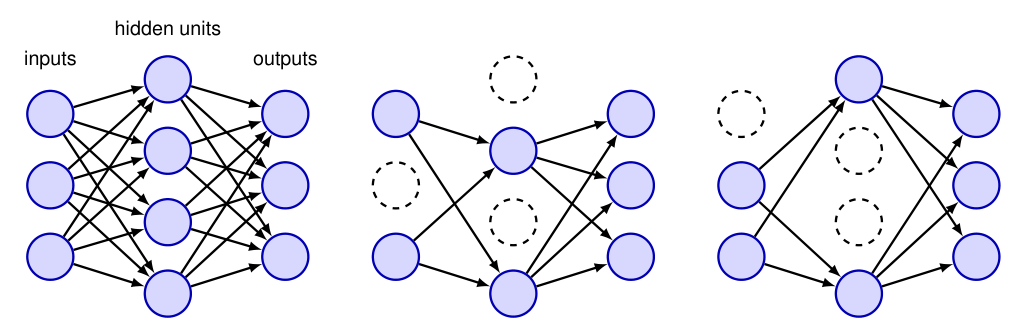
\includegraphics[width=0.8\textwidth]{figure-9-17.png}
% \label{fig:9.17}
\end{figure}

\noindent\rule{\linewidth}{0.4pt}

\section{P9}

Dropout is applied to both hidden nodes and input nodes, but not outputs, and is equivalent to setting the output of a dropped node to zero. It can be implemented by defining a mask vector $R_i \in \{0, 1\}$ which multiplies the activation of the non-output node $i$ for data point $n$, whose values are set to 1 with probability $\rho$. A value of $\rho = 0.5$ seems to work well for the hidden nodes, whereas for the inputs a value of $\rho = 0.8$ is typically used.

\noindent\rule{\linewidth}{0.4pt}

\section{P10}

During training, as each data point is presented to the network, a new mask is created, and the forward and backward propagation steps are applied on that pruned network to create error function gradients, which are then used to update the weights, for example by stochastic gradient descent. If the data points are grouped into mini-batches then the gradients are averaged over the data points in each mini-batch before applying the weight update. For a network with $M$ non-output nodes, there are $2^M$ pruned networks, and so only a small fraction of these networks will ever be considered during training. This differs from conventional ensemble methods in which each of the networks in the ensemble is independently trained to convergence. Another difference is that the exponentially many networks that are implicitly being trained with dropout are not independent but share their parameter values with the full network, and hence with each other. Note that training can take longer with dropout since the individual parameter updates are very noisy. Also, because the error function is intrinsically noisy, it is harder to confirm that the optimization algorithm is working correctly just by looking for a decreasing error function during training.

\noindent\rule{\linewidth}{0.4pt}

\section{P11}

Once training is complete, predictions can in principle be made by applying the ensemble rule (9.42), which in this case takes the form
\begin{equation}
p(\mathbf{y}|\mathbf{x}) = \sum_{\mathbf{R}} p(\mathbf{R}) p(\mathbf{y}|\mathbf{x}, \mathbf{R})
\tag{9.51}
\end{equation}
where the sum is over the exponentially large space of masks, and $p(\mathbf{y}|\mathbf{x}, \mathbf{R})$ the predictive distribution from the network with mask $\mathbf{R}$. Because this summation is intractable, it can be approximated by sampling a small number of masks, and in practice, as few as 10 or 20 masks can be sufficient to obtain good results. This procedure is known as \textit{Monte Carlo dropout}.

\noindent\rule{\linewidth}{0.4pt}

\section{P12}

An even simpler approach is to make predictions using the trained network with no nodes masked out, and to re-scale the weights in the network so that the expected input to each node is roughly the same during testing as it would be during training, compensating for the fact that in training a proportion of the nodes would be missing. Thus, if a node is present with probability $\rho$ during training, then during testing the output weights from that node would be multiplied by $\rho$ before using the network to make predictions.

\noindent\rule{\linewidth}{0.4pt}

\section{P13}

A different motivation for dropout comes from the Bayesian perspective. In a fully Bayesian treatment, we would make predictions by averaging over all possible $2^M$ network models, with each network weighted by its posterior probability. Computationally, this would be prohibitively expensive, both during training when evaluating the posterior probabilities and during testing when computing the weighted predictions. Dropout approximates this model averaging by giving an equal weight to each possible model.

\noindent\rule{\linewidth}{0.4pt}

\section{P14}

Further intuition behind dropout comes from its role in reducing over-fitting. In a standard network, the parameters can become tuned to noise on individual data points, with hidden nodes becoming over-specialized. Each node adjusts its weights to minimize the error, given the outputs of other nodes, leading to co-adaptation of nodes in a way that might not generalize to new data. With dropout, each node cannot rely on the presence of other specific nodes and must instead make useful contributions in a broad range of contexts, thereby reducing co-adaptation and specialization. For a simple linear regression model trained using least squares, dropout regularization is equivalent to a modified form of quadratic regularization.

\end{document}
